\documentclass{standalone}
\usepackage{graphicx}	
\usepackage{amssymb, amsmath}
\usepackage{color}

\usepackage{tikz}
\usetikzlibrary{intersections, backgrounds}
\usepackage{pgfmath}

\definecolor{light}{RGB}{220, 188, 188}
\definecolor{mid}{RGB}{185, 124, 124}
\definecolor{dark}{RGB}{143, 39, 39}
\definecolor{highlight}{RGB}{180, 31, 180}
\definecolor{gray10}{gray}{0.1}
\definecolor{gray20}{gray}{0.2}
\definecolor{gray30}{gray}{0.3}
\definecolor{gray40}{gray}{0.4}
\definecolor{gray60}{gray}{0.6}
\definecolor{gray70}{gray}{0.7}
\definecolor{gray80}{gray}{0.8}
\definecolor{gray90}{gray}{0.9}
\definecolor{gray95}{gray}{0.95}

\newcommand*{\offset}{0.025}

\begin{document}

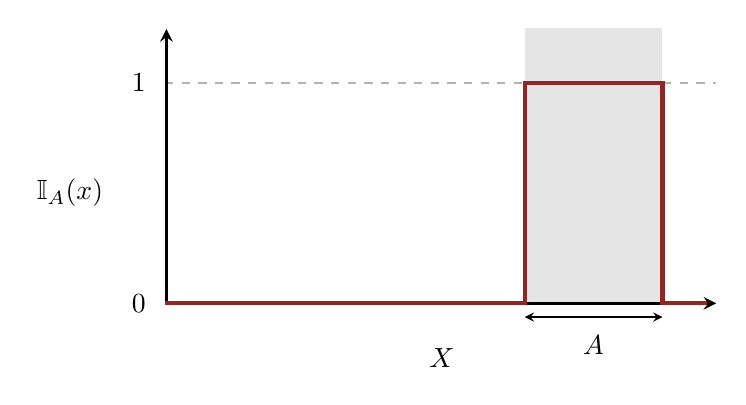
\begin{tikzpicture}[scale=0.35, thick]

  \node[] at (-3.5, 4) { $\mathbb{I}_{A}(x)$ };

  \fill[color=gray90] (13, 0) rectangle (18, 10);
  \draw [<->, >=stealth, line width=0.5] (13, -0.5) -- (18, -0.5);
  \node[] at (15.5, -1.5) { $A$ };

  \draw [dashed, color=gray70] (-0.05, 8) -- +(20, 0);
  \node[] at (-1, 0) { $0$ };
  \node[] at (-1, 8) { $1$ };

  \draw [->, >=stealth, line width=1] (-0.05, 0) -- +(20, 0);
  \draw [->, >=stealth, line width=1] (0, -0.05) -- +(0, 10);
  \node[] at (10, -2) { $X$ };
  
  \draw [color=dark, line width=1.5] (-0.05, 0) -- (13, 0) -- (13, 8) -- (18, 8) -- (18, 0) -- (19.6, 0);
   
\end{tikzpicture}

\end{document}  